\chapter*{Introduction}
\addcontentsline{toc}{chapter}{Introduction}

Dans le cadre du module de projet informatique du second semestre de L2, nous avons développé une application permettant la synchronisation et la répartition des données d'un utilisateur entre plusieurs services de stockage dans les nuages.

Notre groupe est composé de deux personnes, Rémi \textsc{Cérès} et Mattéo \textsc{Delabre}, et nous sommes encadrés par Mme Hinde \textsc{Bouziane}. La réalisation du projet s’est déroulée sur une période de 15~semaines, de
janvier à mi-mai 2017.

\section*{Motivations du projet}

Le stockage de données dans les nuages consiste pour un utilisateur à confier ses données à un service qui s'occupe de les stocker pour lui, et de les lui restituer dès qu'il en a besoin. Un tel service est généralement opéré par une entreprise qui est responsable de l'intégrité des informations déposées.

Ce mode de stockage offre de nombreux avantages, permettant par exemple à l'utilisateur d'accéder à ses données depuis plusieurs appareils, de conserver une copie de sauvegarde de celles-ci, voire d'en partager certaines avec d'autres personnes. Ce modèle s'est considérablement développé ces dernières années, et diverses entreprises telles que Amazon, Google ou Microsoft proposent de stocker gratuitement les données de leurs utilisateurs.

Malgré les nombreux avantages du stockage dans les nuages, il cause une centralisation des données de l'utilisateur sur un seul service et une dépendance sur celui-ci. L'utilisateur place en effet ses données entre les mains d'une unique entreprise, et par ailleurs sa confiance dans la bonne gestion de ses informations par cette entreprise.

Cette centralisation le fait dépendre du service et de la société qui le gère, qui peut à tout moment décider de modifier son offre ou d'y mettre fin. Les services gratuits n'offrent par ailleurs souvent aucune garantie quant à la confidentialité des données déposées.

\section*{Objectifs du projet et cahier des charges}

Nous avons baptisé notre projet Arcus, en référence au nuage bas du même nom, qui prend la forme d'un tube et est souvent associé aux \emph{cumulus} et \emph{cumulonimbus}. L'objectif est de permettre à un utilisateur de synchroniser les répertoires de son choix entre sa machine et différents services de stockage dans les nuages. En agissant comme un tube qui ferait le lien entre ces différents services, il se veut une réponse aux problématiques énoncées précédemment.

Cet objectif est donc similaire à celui d’autres applications de synchronisation comme celle de Dropbox, Nextcloud ou Apple, mais se distingue notamment par le fait que les données soient réparties sur différents services au contraire des moteurs de synchronisation classiques qui ne les synchronisent qu'avec un service particulier.

Nous avons décidé du cahier des charges suivant pour notre application.

\begin{description}
    \item[Interface commune aux services de stockage dans les nuages.] Notre application sera indépendante des services utilisés. Habituellement, chaque fournisseur de service propose sa propre application de synchronisation. Dans le cas où l'utilisateur se sert de plusieurs services, il doit installer plusieurs applications ayant le même but. Un objectif pour notre outil est de pouvoir fonctionner avec le plus de services différents possibles.
    \item[Répartition des données de l'utilisateur.] Chaque fichier déposé par l'utilisateur dans un des répertoires choisis sera découpé en plusieurs blocs, qui seront envoyés sur différents services de stockage existants. Dans le cas où un de ces services serait ajouté ou supprimé, les données seraient alors redistribuées afin que toutes les informations restent accessibles. Cette répartition se fera de telle sorte que le service avec le plus d'espace libre soit priorisé, afin d'équilibrer au mieux l'espace occupé sur chaque service.
    \item[Réplication des données de l'utilisateur.] Les blocs de données seront stockés de manière redondante sur au moins deux services différents quand cela sera possible. Cela permettra de se prémunir d'une panne d'un des services dépositaires ou de tout événement entraînant une perte de l'accès aux données.
    \item[Chiffrement des données de l'utilisateur.] Avant de transmettre les blocs de données aux serveurs, ceux-ci seront chiffrés. Ce chiffrement garantira la confidentialité des données de l'utilisateur puisqu'il empêchera les services dépositaires et toute autre personne tierce d'accéder au contenu des blocs.
    \item[Transparence de fonctionnement de l'application.] Les opérations de synchronisation, de répartition et de chiffrement des données s'exécuteront en fond. Les interactions directes avec l'utilisateur se limiteront à la gestion des fichiers par l'intermédiaire de l'explorateur de fichiers, à la résolution de conflits éventuels et à la configuration de l'application.
\end{description}

Notre application permettra ainsi de réduire le risque de perte des données de l'utilisateur en les répartissant et en les répliquant à travers plusieurs fournisseurs de services de stockage. En combinant ce mécanisme de répartition au chiffrement, elle accroîtra la confidentialité de ces données. Enfin, elle permettra de fédérer l'accès à plusieurs services en une seule application et de bénéficier des ressources de stockage de plusieurs fournisseurs combinés.

\noindent
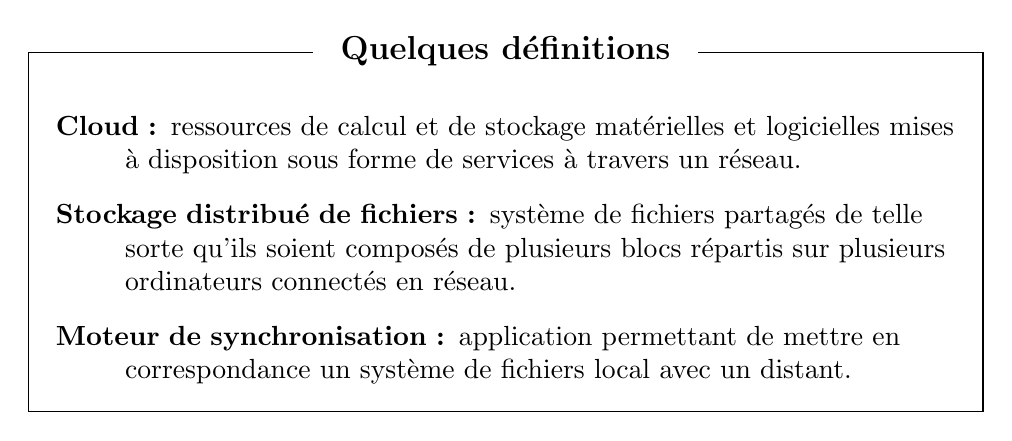
\begin{tikzpicture}
\node [text width=\textwidth - 20pt, draw, inner sep=10pt]
    (definitions) {
        \begin{description}
            \item[Cloud :] ressources de calcul et de stockage matérielles et logicielles mises à disposition sous forme de services à travers un réseau.
            \item[Stockage distribué de fichiers :] système de fichiers partagés de telle sorte qu'ils soient composés de plusieurs blocs répartis sur plusieurs ordinateurs connectés en réseau.
            \item[Moteur de synchronisation :] application permettant de mettre en correspondance un système de fichiers local avec un distant.
        \end{description}
    };
\node [fill=white, inner xsep=10pt] at (definitions.north)
    {\textbf{\large Quelques définitions}};
\end{tikzpicture}

Dans un premier temps, nous présenterons les méthodes et outils de travail que nous avons adoptés pour organiser ce projet. Ensuite, nous détaillerons la modélisation que nous avons choisie pour l'application, puis les technologies utilisées pour son implémentation. Enfin, nous ferons le point sur l'avancement du projet, les difficultés que nous avons rencontrées jusqu'ici et les perspectives qui s'offrent à nous pour la poursuite du développement d'Arcus.
